\begin{frame}
  \frametitle{Repository Layouts}

  \begin{minipage}{0.49\textwidth}
    \begin{figure}[h!]
      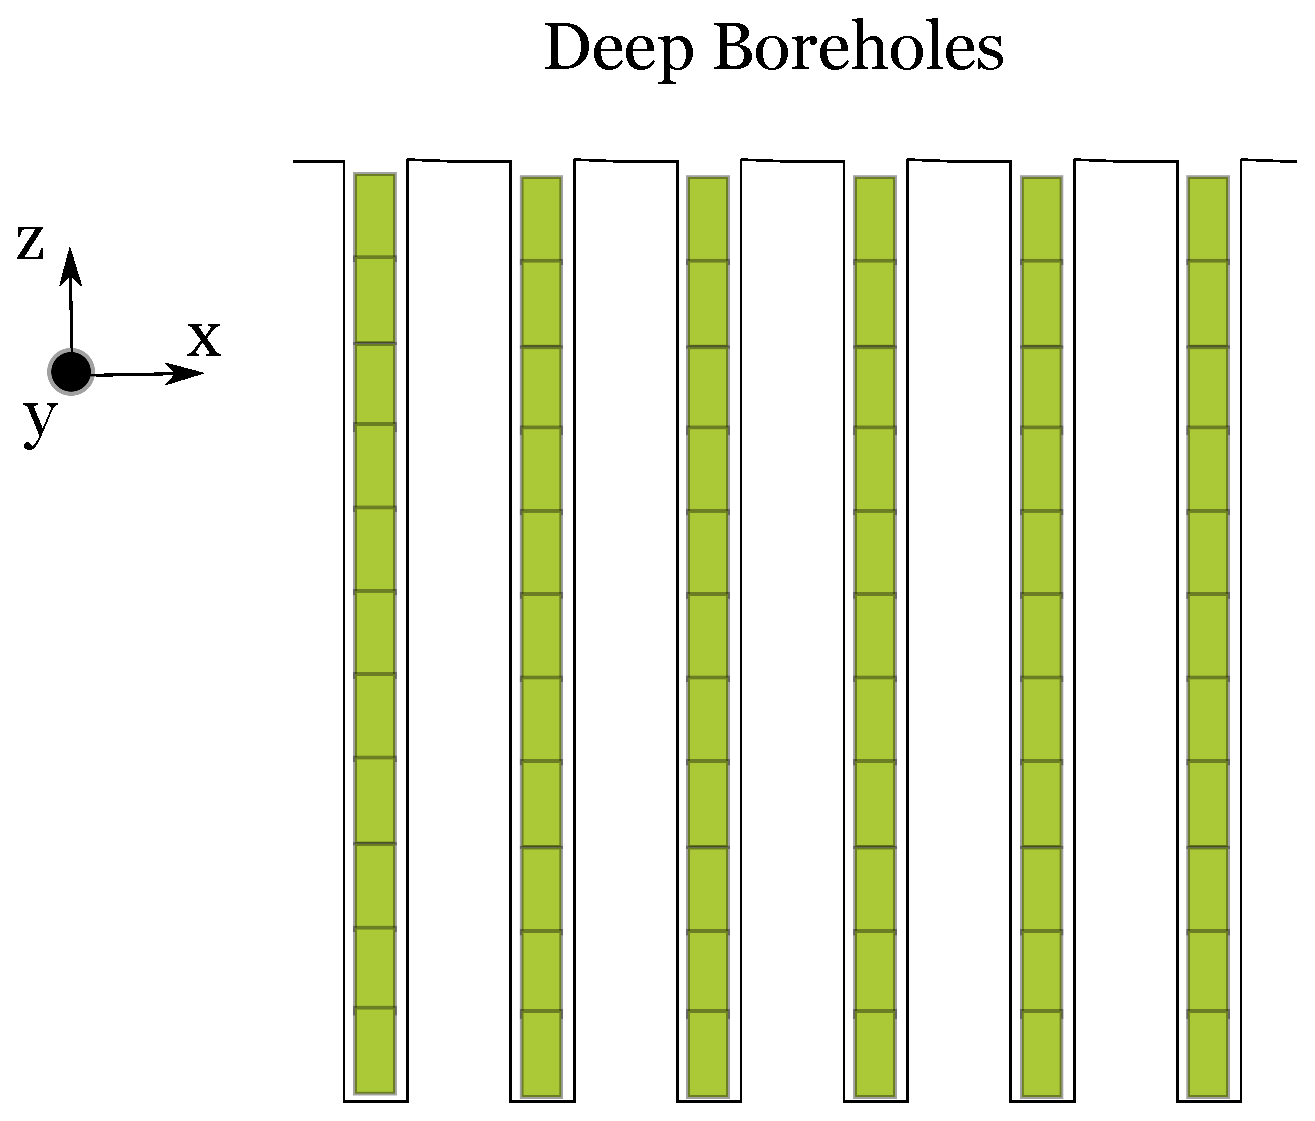
\includegraphics[width=0.75\textwidth]{boreholes.eps}
    \end{figure}
    \begin{figure}[h!]
      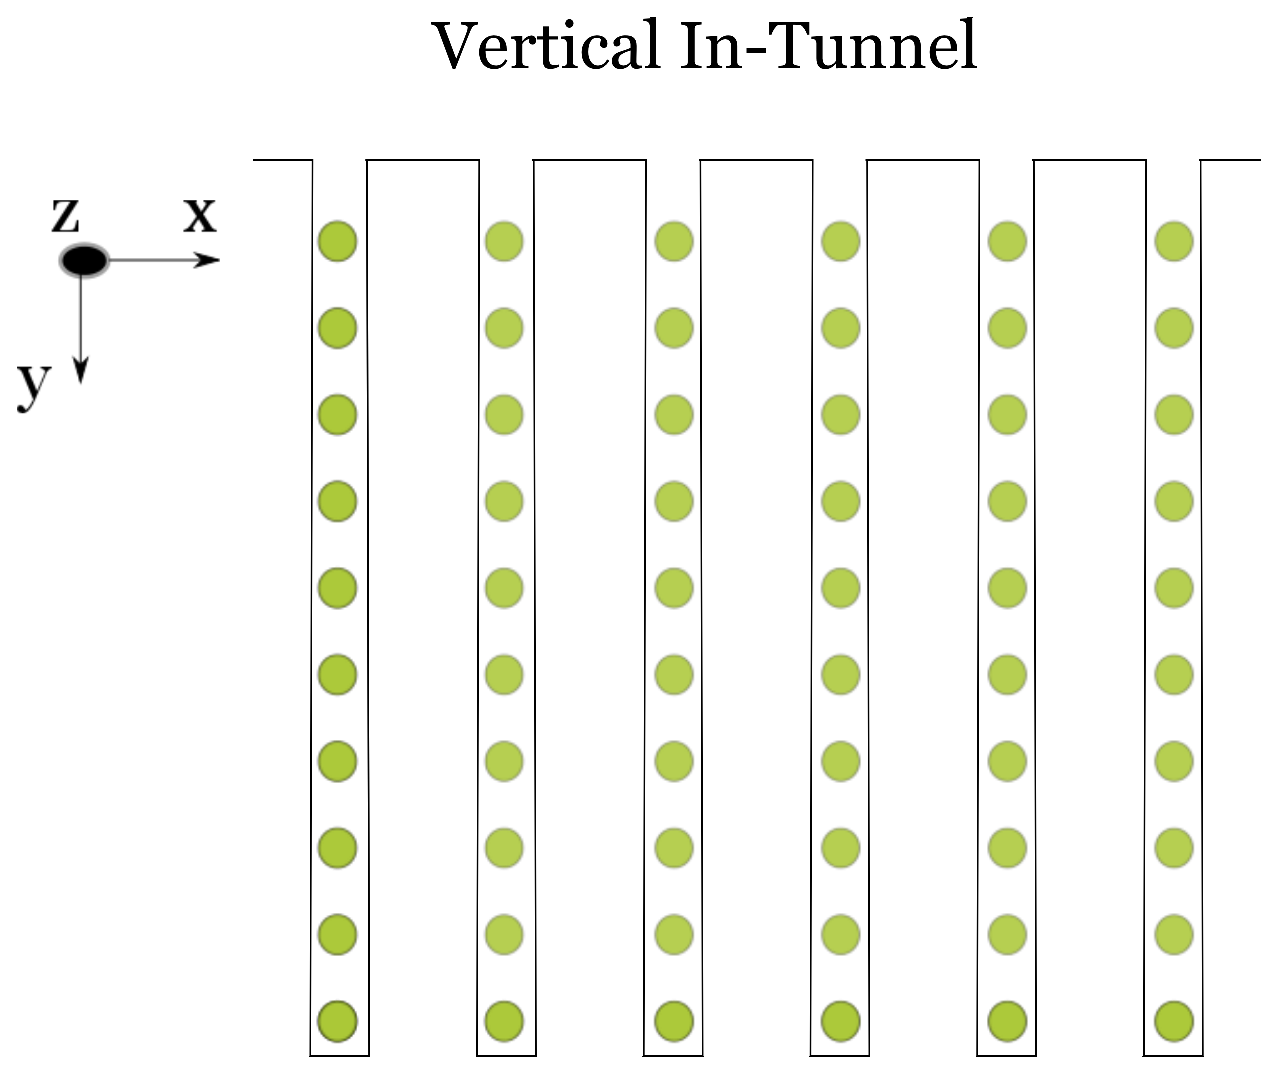
\includegraphics[width=0.75\textwidth]{vertical.eps}
    \end{figure}
  \end{minipage}
  \hspace{0.01cm}
  \begin{minipage}{0.49\textwidth}
    \begin{figure}[h!]
      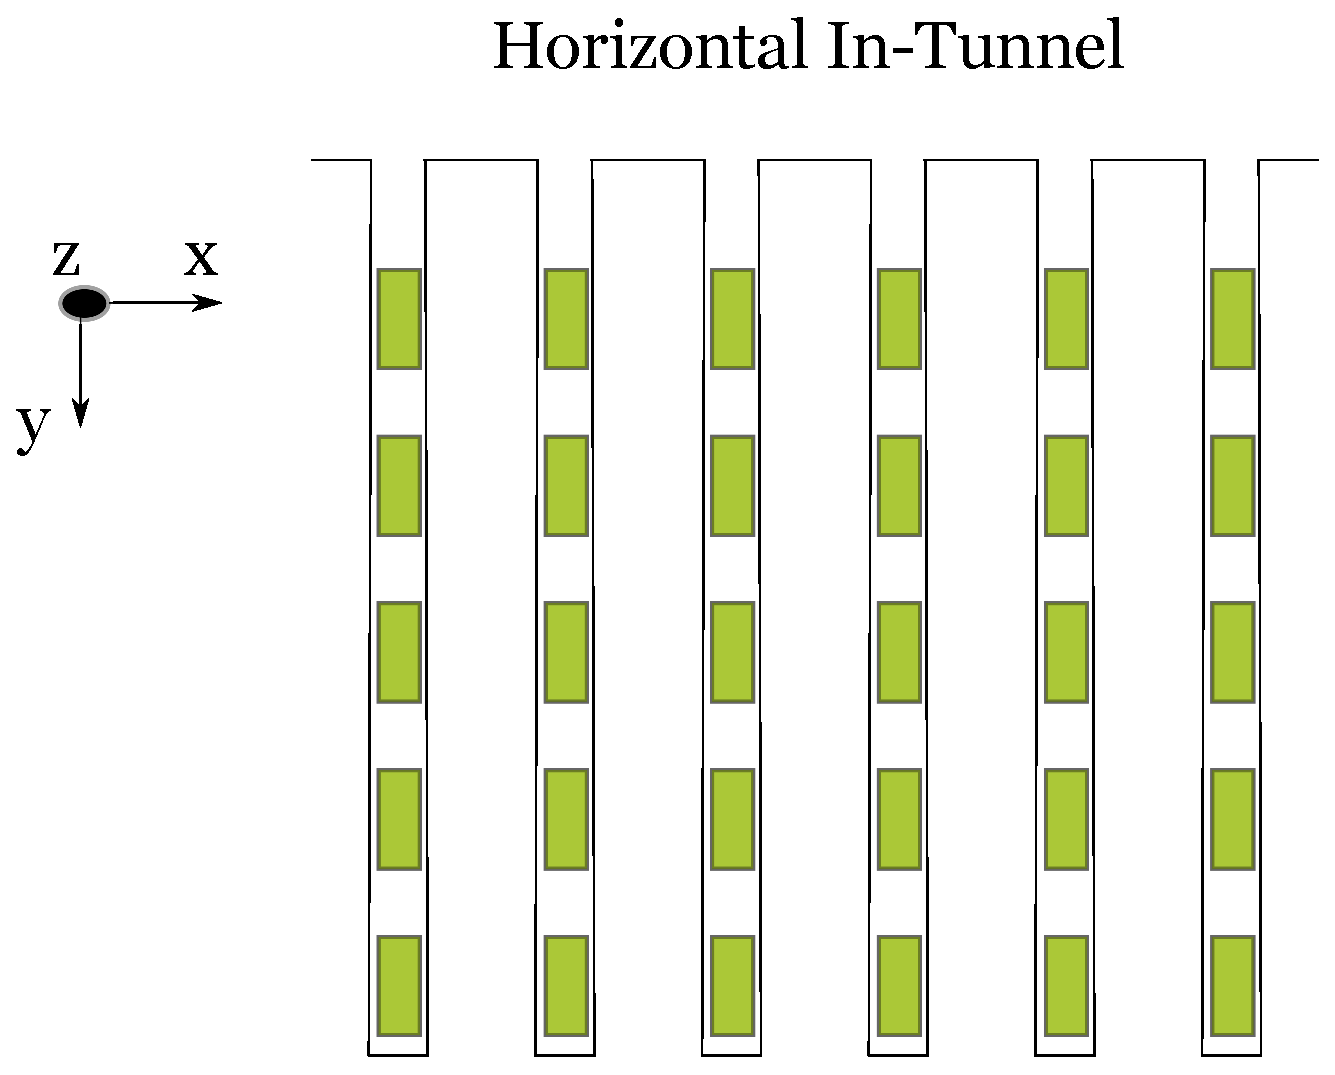
\includegraphics[width=0.8\textwidth]{horizontal.eps}
    \end{figure}
    \begin{figure}[h!]
      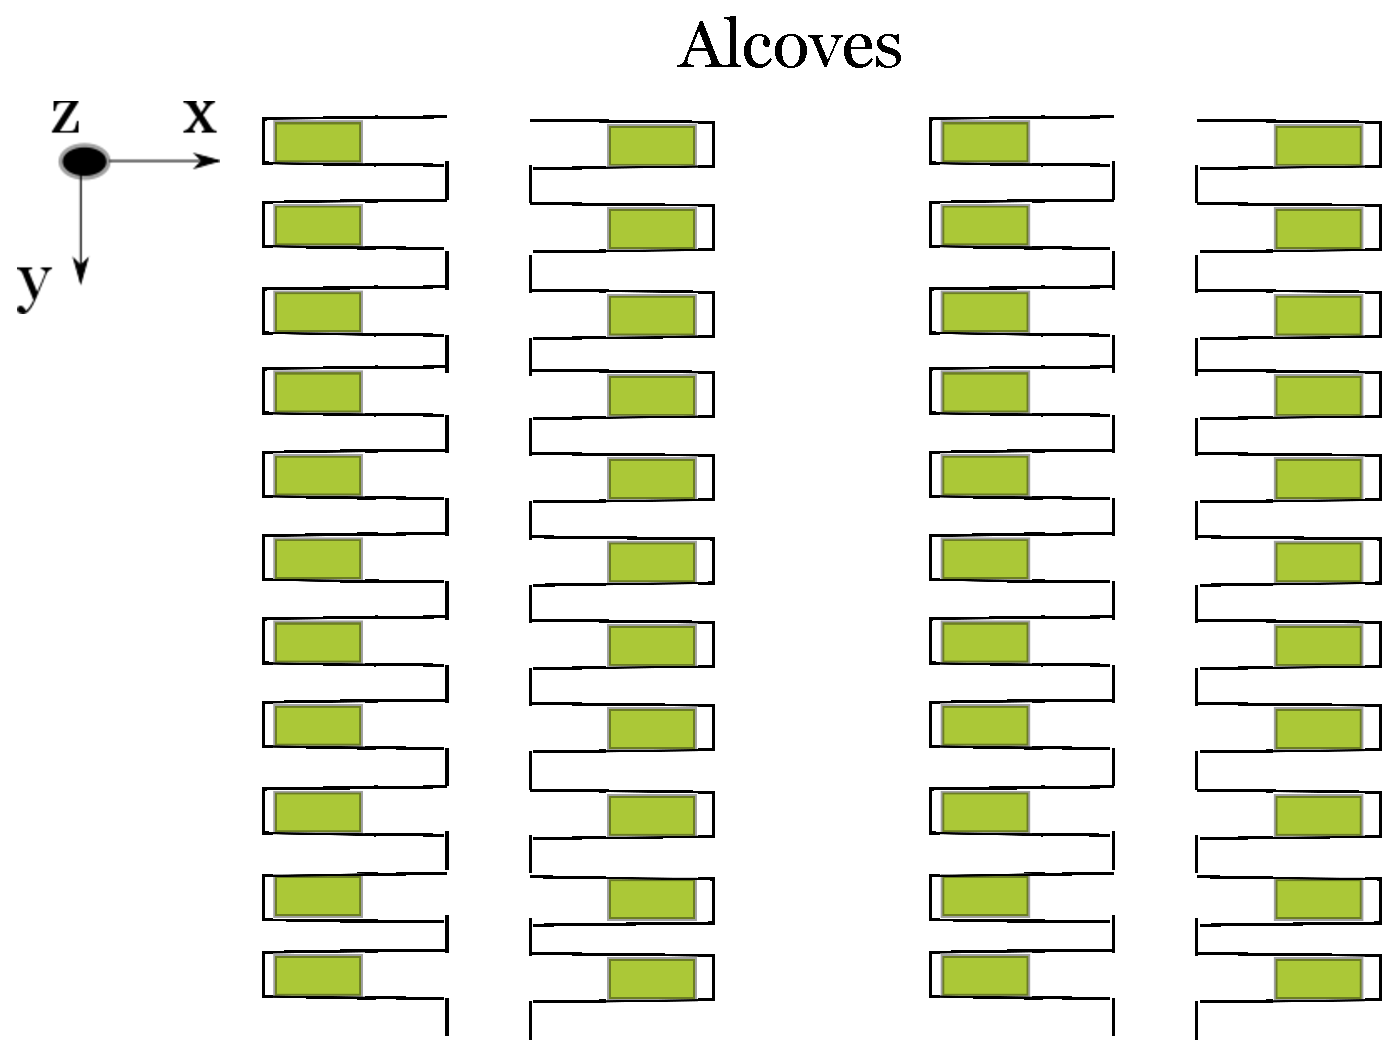
\includegraphics[width=0.8\textwidth]{alcoves.eps}
    \end{figure}
  \end{minipage}

\end{frame}

\begin{frame}[ctb!]
  \footnotesize{
  \frametitle{Unsaturated, Ventilated Concepts}
  \begin{figure}[htbp!]
  \begin{center}
    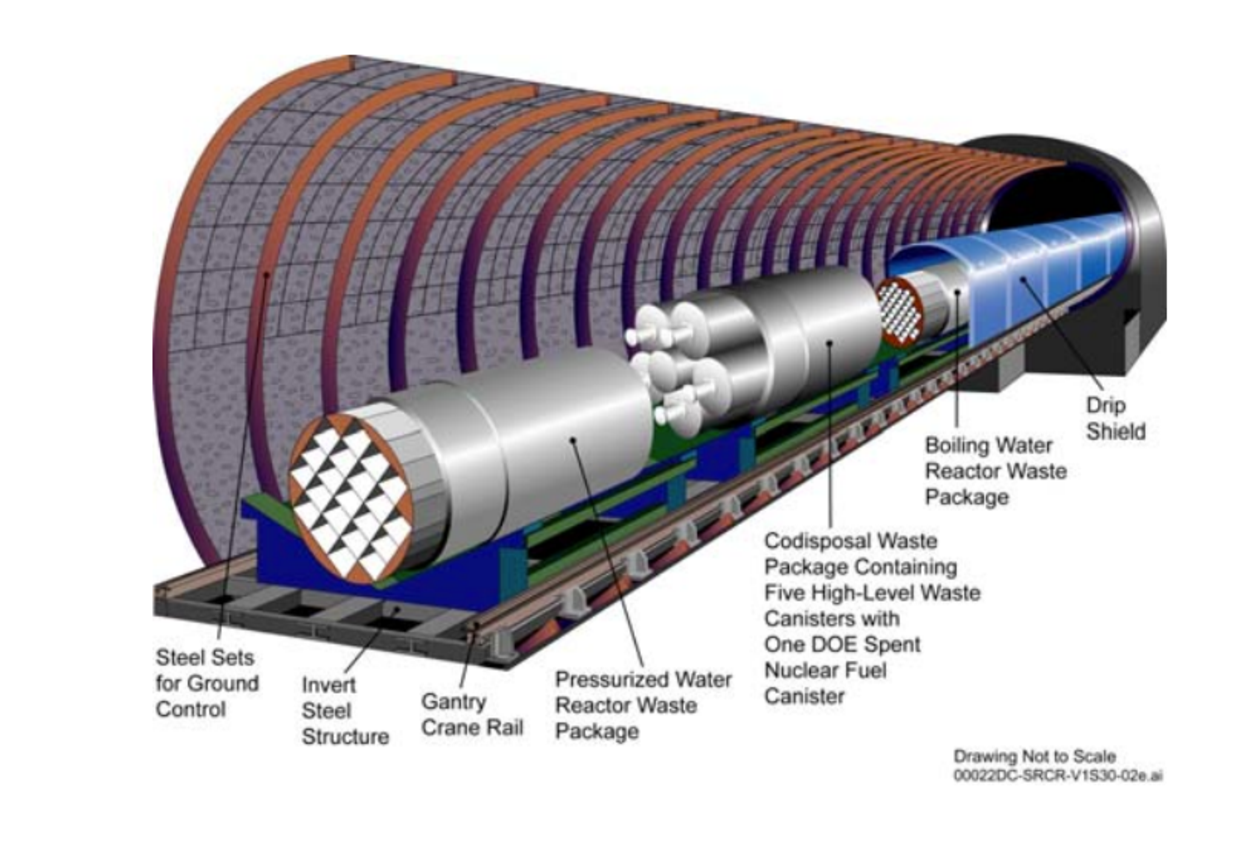
\includegraphics[height=0.7\textwidth]{yucca_tunnel.eps}
  \end{center}
  \caption{The current U.S. geologic disposal concept \cite{peters_whats_2013}.}
  \label{fig:yucca_tunnel}
\end{figure}

}
\end{frame}

\begin{frame}[ctb!]
  \footnotesize{
  \frametitle{Saturated , Enclosed Concepts} 
 \begin{figure}[h!]
    \begin{center}
      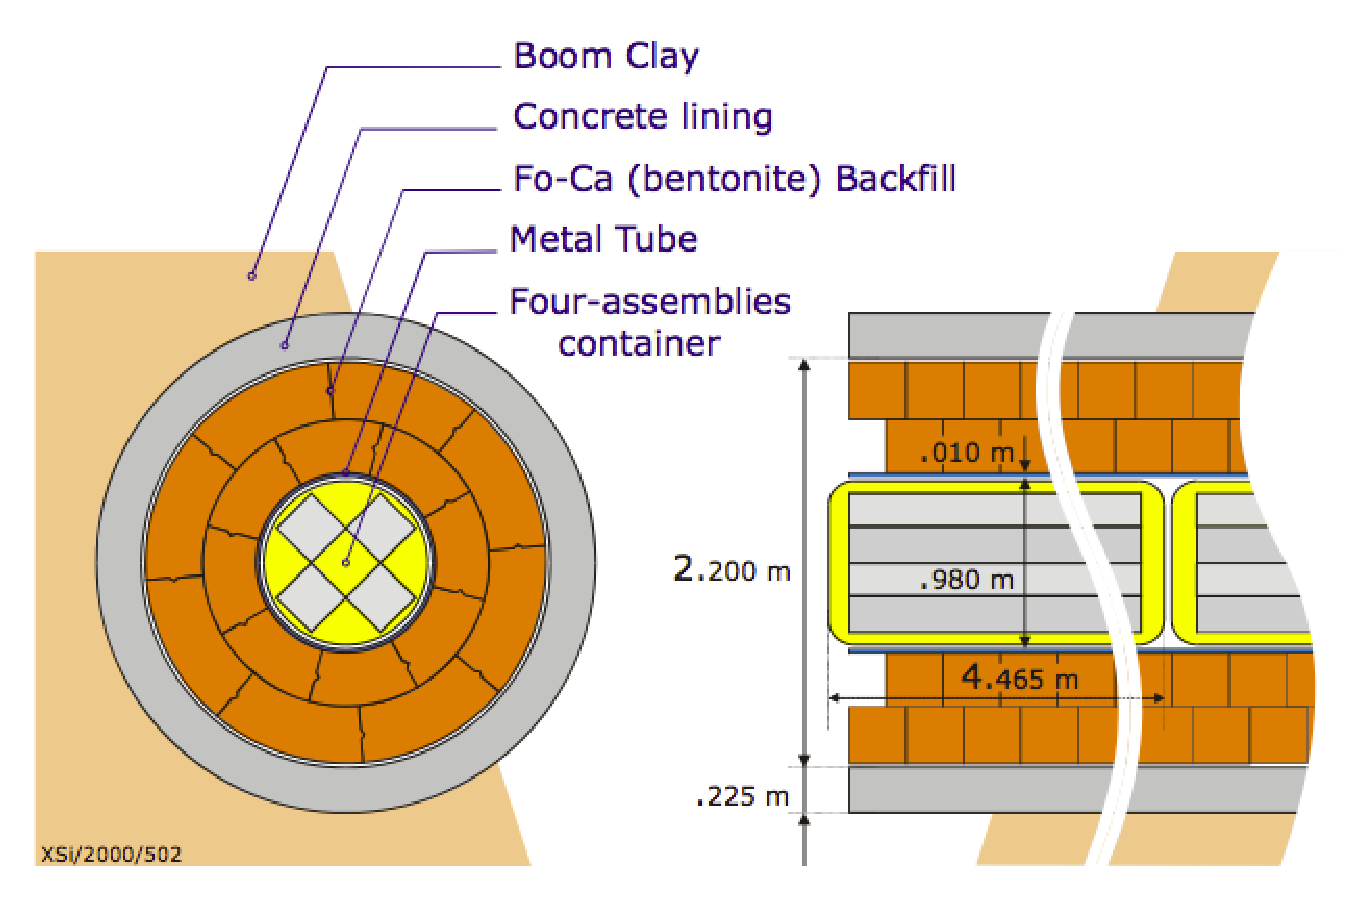
\includegraphics[height=.7\textheight]{belgianClayRedImp.eps}
    \end{center}
    \caption{The Belgian reference concept in Boom Clay is backfilled very soon
   after waste emplacement without a ventilation period and is located below the water table
   \cite{von_lensa_red-impact_2008}.}
    \label{fig:belgianClayRedImp}
  \end{figure}
}
\end{frame}
